\section{Body Chapter: Paradigm Induction}
\label{sec:inflection}

The study proposed in this section will leverage IGT and machine learning 
%to learn inflectional paradigms. 
to predict inflected word forms in six languages. 
%Human annotation for NLP is considered expensive because it relies so much on language domain expertise \cite{buys_cross-lingual_2016}. For documentary and descriptive linguistics, employing this expertise is a long accepted practice. The workflow is conducted in close cooperation with native speakers. A language's inflectional morphology is studied partly from the information in IGT. 
Patterns of inflectional morphology, or inflectional paradigms, are described as tables. The tables may illustrate a paradigms with the inflectional affixes, as in Table \ref{tab:EngParadigm} in Chapter \ref{chap:litreview}, or with an example lexeme, as in Table \ref{tab:RuParadigm}. Paradigm tables are featured in published grammatical descriptions, used for language learning, and serve as NLP resources in projects such as UniMorph \cite{kirov_unimorph}. 
%and partly by eliciting  from native speakers. 
%Inflectional paradigms inflectional paradigms is an example of descriptive linguistic analysis that informs our understanding of human language, 
As with most descriptive work, documenting and describing a language's paradigms is done with very little automated assistance. 
%This bottlenecks the production of descriptive resources for thousands of under-described languages, even languages with over a million speakers, such as Manipuri in India. 

\begin{table}
\begin{center}
\begin{tabular}{c|c|c|c|c|c|c}
{} & \multicolumn{2}{c|}{\bf Class 1} & \multicolumn{2}{c|}{\bf Class 2} & \multicolumn{2}{c}{\bf Class 3} \\
\cline{2-7}
{}    & \textsc{sg} & \textsc{pl}    & \textsc{sg} & \textsc{pl} & \textsc{sg} & \textsc{pl} \\
\hline
\textsc{nom} & -a & -\textbari & \O & -\textbari & -\textsuperscript{j} & -i \\
\textsc{acc} & -u & -\textbari /\O  & \O/-a & -\textbari/-ov & -\textsuperscript{j} & -i/-jej \\
\textsc{gen} & -\textbari & \O & -a & -ov & -i & -jej \\
\textsc{dat} & -je & -am & -u & -am & -i & -jam \\
\textsc{inst} & -oj & -ami & -om & -ami & -ju & -jami \\
\textsc{prep} & -je & -ax & -je & -ax & -i & -jax \\
\end{tabular}
\caption[Inflectional Paradigms for Russian Nouns]{Inflectional Paradigms for Russian Nouns. 
%The second row and leftmost column indicate the morphosyntactic features that each slot represents.
}
\label{tab:RuParadigm}
\end{center}
\end{table}

This study will investigate whether manual preprocessing of paradigms extracted from IGT data improves machine learning performance. The task is \textbf{IGT-to-paradigms} (IGT2P). It is illustrated in Figure \ref{fig:IGT2PWorkflow}. IGT2P can be seen as a noisy version of morphological \textit{re}inflection \cite{cotterell_sigmorphon_2016}. It differs from previous computational morphological inflection tasks \cite{yarowsky-wicentowski-2000-minimally,faruqui-etal-2016-morphological} in two aspects: (1) paradigms extracted from IGTs are noisier than curated training data that is normally used and (2) part-of-speech (POS) tags that are typically part of the models are often unavailable in documentary data. Adding POS tags is usually a later step, after translation, morpheme segmentation, and glossing. Therefore, a secondary question this study is whether Part-of-speech (POS) tags are necessary for the task. 

\begin{figure}[h!]
    \begin{center}
    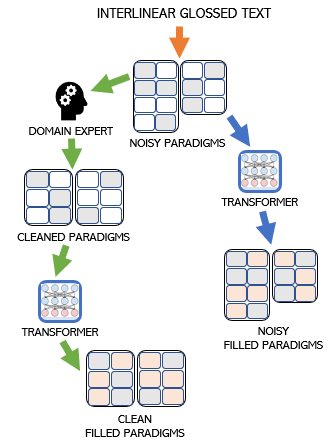
\includegraphics[width=8cm]{figs/IGT-Paradigm-Workflow.png}
    \caption[IGT2P Workflow]{IGT2P Workflow. 
    %Inflected word forms attested in interlinear glossed texts (IGT) train transformer encoder-decoder to generalize morphological paradigmatic patterns and generate word forms when given known morphosyntatic features of missing paradigm cells. Noisy paradigms are automatically constructed from IGT and a language expert creates ``cleaned'' paradigms. Both sets are tested on the same missing word forms and the results are compared.
    }
    \label{fig:IGT2PWorkflow}
    \end{center}
\end{figure}

%Supervised inflection tasks require complete or partially complete paradigm tables as training data. These tables are challenging to induce from raw data. The patterns of a langauge's various inflectional patterns are often irregular. They may have overlapping patterns and isomorphic morphemes that result in ambiguous forms. 
%For example, an Arapaho verb ending in \textit{-\'ot} might mean ``You alone do something to \underline{him/her/it}'' or it might mean ``You alone do something to \underline{them}.'' Some languages use suppletive forms that have no similarity in shape to their ``base'' form (as in the English ``to be'' verb in Table \ref{tab:EngParadigm}). 

Besides the lack of POS tags, several issues must be considered. Most notably, IGTs contain noise. 
%One reason for this is the dynamic nature of ongoing linguistic analysis. 
As the linguist gains a better understanding of the language's structure during interlinearization, morpheme boundaries and glosses at the beginning of a corpus may differ from later ones. 
%Also, IGTs are rarely complete because a linguist may be focusing on one particular phenomenon under investigation. 
%For example, in Manipuri, sometimes only one morphosyntactic feature was glossed on each token, resulting in several different inflected forms in a paradigm having the same morphosyntactic features. 
%Another issue is the annotation quality. 
Noise also arises from human errors or choices made for the sake of convenience. This can be caused by factors such as how the annotators were trained, how much linguistic knowledge they had, how careful the annotators were, how much time was spent correcting errors and inconsistencies, and whether the documentary team considered the inconsistencies significant.
%because the tedious process is performed primarily by hand. 
For example, different stem morphemes may be glossed with the same English word. Lezgi has several copula verbs which can be narrowly translated as `be in', `be at', etc., but many occurrences in the data were merely glossed as `be'. The distinction is clear when in the context of the IGT, but for the pilot study, it meant that all forms of all these lemmas were initially grouped into one paradigm.  
    
The selected corpora do not differentiate between derivational and inflectional morphemes; thus, this study will not rigorously distinguish between them either. The same is true for clitics. This means that the morphological patterns that the model learns will not always, strictly speaking, be part of inflectional paradigms, It does mean that the model is learning all possible ``words'' that can be formed from one lemma.

\paragraph{Step 1: Preprocessing paradigms.}
As a first step, partial inflectional paradigms will be automatically extracted from the IGT. Words will be organized into paradigms based on the gloss of the stem morpheme. Then these stem glosses are removed, leaving only the affix glosses which are treated as the lexeme's morphosyntactic features. These features dictate a lexeme's inflection.

The automatically extracted paradigms will be preprocessed in two ways. In the first method, language domain experts will be asked to ``clean up'' the automatically extracted paradigms. Experts will be asked to spend no more than six hours on the cleaning task. They will reorganize words into correct inflectional paradigms, for example, by regrouping Lezgi copula verbs. They will also complete missing morphosyntatic information; for example, adding PL (plural) or SG (singular) to nouns that are otherwise glossed identically. Finally, they will remove any words that are morphologically derived from another part of speech but not morphologically inflected. For example, an affix might derive an adverb from a noun root, and if the adverbializing affix was clearly glossed, then that word form will have been extracted automatically. This would result in more noise since it displays derivational morphology and no inflectional morphology. Experts will remove words thes non-inflected words.

For the second preprocessing method, the automatically extracted paradigms will be eyeballed by a non-expert. Since non-experts can not be expected to identify and correct most issues, they will simply remove obvious mistakes and inconsistencies. These include identical words with different glosses or different words with identical glosses.

%EXAMPLE OF CLEAN VS UNCLEANED DATA?

\paragraph{Step 2: Preparing training data.}
The typical morphological reinflection data is in tuple format of \texttt{(source form, target form, target features)}. The extracted paradigms will be converted into this format. Each word form will be first mapped to itself, then to every other form in its paradigms, and added to the training data. Paradigms with a single entry will have only self-to-self mapping. 

For both sets of paradigms, two methods for augmenting limited training data will be prepared. The first method will augment data with artificial word forms. The second will augment with all the uninflected or unannotated tokens in the IGT. A third training set will be prepared that combines the two methods.

The validation and test sets will be prepared from the expert-cleaned data language in the following way: If the paradigm has more than one form, pick a random form as the source form and select the remaining forms in the paradigm with a probability of 0.3 to be ``unknown'', i.e. to be predicted from the first form. Half of the ``unknown'' data transformed in this way will be used for validation and the other half for testing. The validation and test sets for each language will be shared across all experiments.
 
\paragraph{Step 3: Reinflection models and experimental setup.}
After paradigms are extracted and prepared, two experiments will generate ``unknown'' inflected forms. One will be run on a Transformer and the other on a LSTM sequence-to-sequence model with exact hard monotonic attention for character-level transduction. Both models will have the same implementation and hyperparameters as the SIGMORPHON 2020 shared task 0 baseline \cite{vylomova2020sigmorphon}.\footnote{\url{https://github.com/shijie-wu/neural-transducer/tree/f1c89f490293f6a89380090bf4d6573f4bfca76f}} Both models will be tested on the same held-out set of morphosyntactic features chosen randomly from paradigms that are not single-entry. 

The study will compare the performance of the models trained on the noisy paradigms to performance on the expertly cleaned paradigms and across the three data augmentation methods. The results will show whether the integration of manual work improves results. It will also indicate how performance varies according to IGT quality.  

\subsection{Pilot Study: IGT2P}
\label{sec:pilotIGT2P}

This section summarizes an IGT2P pilot study on Lezgi. A fuller description is under review at EMNLP 2020. It shows that IGT2P is a promising method for integrating machine learning into the documentation and description of morphological inflection patterns.
%for the creation of morphological resources in low-resource languages and might be integrated into morphological analysis in order to speed and improve a linguist's work.

\begin{table}[t]
\centering
    \begin{tabular}{l|cccc|cccc}
    \toprule
      \textbf{} & \textbf{T} & \textbf{+aug} & \textbf{+uninfl} & \textbf{+both} & \textbf{mono} &  \textbf{+aug} &
      \textbf{+uninfl} &
      \textbf{+both} \\
       %\hline
      %arp clean & \textbf{62.08} & 61.39 & 61.58 & 60.78 & 15.93 & 15.75 & 15.58 & 15.94 \\
      %arp noisy & 57.77 & 57.64 & \textit{58.04} & 57.51 & 14.51 & 14.64 & 14.52 & 14.69 \\
      %\midrule
      %btz clean & 7.69 & 3.85 & 1.92 & 1.92 & 1.92 & 5.77 & 1.92 & 1.92  \\
      %btz noisy & 9.62 & 9.62 & \textit{13.46} & 3.85 & 5.77 & 13.46 & 1.92 & \textbf{17.31}  \\
      %\midrule
      %ddo clean & 65.38 & \textbf{66.53} & 65.19 & 65.42 & 59.9 & 60.87 & 59.53 & 60.64  \\
      %ddo noisy & 63.54 & 63.95 & 62.89 & \textit{64.04} & 59.12 & 58.66 & 57.87 & 57.97 \\
      \hline
      lez clean & 46.59 & 32.95 & 46.59 & \textbf{48.86} & 32.95 & 35.23 & 31.82 & 31.82 \\
      lez noisy & \textit{35.23} & 29.55 & 32.95 & 27.27 & 30.68 & 28.41 & 20.45 & 31.82 \\
      %\hline
      %mni clean & 30.63 & 30.87 & 31.81 & \textbf{32.04} & 23.24 & 25.7 & 21.95 & 24.77 \\
      %mni noisy & 21.48 & \textit{22.3} & 21.6 & 21.83 & 18.78 & 18.31 & 19.37 & 20.31 \\
      %\midrule
      %ntu clean & \textbf{53.18} & 46.82 & 49.15 & 48.52 & 29.66 & 33.9 & 28.18 & 33.05 \\
      %ntu noisy & 36.86 & 45.55 & 45.34 & \textit{45.76} & 31.99 & 33.69 & 31.78 & 30.93 \\
    \end{tabular}
    \caption[IGT2P Pilot Study Results]{IGT2P Pilot Study Results. Transformer` (T) and LSTM with exact hard monotonic attention (mono). The addition of artificial data augmention (+aug), unannotated/uninflected word forms (+uninfl), or both. Boldface indicates best overall; italics is best on noisy paradigms.}
    \label{tab:IGT2Presults}
\end{table}
 
Experiments were trained on the inflected forms extracted from the Lezgi IGT. The results are shown in Table \ref{tab:IGT2Presults}. The approximately 18,000 annotated tokens in the Lezgi IGT were sufficient to correctly predict the inflected forms for about one-third of the test data, even without POS tags. It is clear that manual cleaning improved performance and should be tested with more languages. The transformer outperformed the LSTM on both noisy and cleaned data but the difference is not large enough to dispense with the LSTM model in the dissertation research. 
Augmenting the paradigms with artificial data or with uninflected/unannotated tokens lowered performance in most cases. However, augmenting with both improved the Transformer's results on the cleaned data, although by less than half a percent. 
%This makes it unclear whether augmenting the data improves results. 
%It should be noted that the Lezgi IGT annotations are less consistent or complete (i.e. not all morphemes were glossed) than some of the other corpora. 
The proposed dissertation research will experiment with more languages to see whether manual cleaning continues to be a good method for integration and to examine factors that might affect the results.  


%This would be a significant contribution because manual efforts are on the order of months or years in order to  paradigms and then produce the very clean and complete structured data normally used to train NLP morphological models.

